%%
%% This is file `sample-manuscript.tex',
%% generated with the docstrip utility.
%%
%% The original source files were:
%%
%% samples.dtx  (with options: `manuscript')
%% 
%% IMPORTANT NOTICE:
%% 
%% For the copyright see the source file.
%% 
%% Any modified versions of this file must be renamed
%% with new filenames distinct from sample-manuscript.tex.
%% 
%% For distribution of the original source see the terms
%% for copying and modification in the file samples.dtx.
%% 
%% This generated file may be distributed as long as the
%% original source files, as listed above, are part of the
%% same distribution. (The sources need not necessarily be
%% in the same archive or directory.)
%%
%% Commands for TeXCount
%TC:macro \cite [option:text,text]
%TC:macro \citep [option:text,text]
%TC:macro \citet [option:text,text]
%TC:envir table 0 1
%TC:envir table* 0 1
%TC:envir tabular [ignore] word
%TC:envir displaymath 0 word
%TC:envir math 0 word
%TC:envir comment 0 0
%%
%%
%% The first command in your LaTeX source must be the \documentclass command.
%%%% Small single column format, used for CIE, CSUR, DTRAP, JACM, JDIQ, JEA, JERIC, JETC, PACMCGIT, TAAS, TACCESS, TACO, TALG, TALLIP (formerly TALIP), TCPS, TDSCI, TEAC, TECS, TELO, THRI, TIIS, TIOT, TISSEC, TIST, TKDD, TMIS, TOCE, TOCHI, TOCL, TOCS, TOCT, TODAES, TODS, TOIS, TOIT, TOMACS, TOMM (formerly TOMCCAP), TOMPECS, TOMS, TOPC, TOPLAS, TOPS, TOS, TOSEM, TOSN, TQC, TRETS, TSAS, TSC, TSLP, TWEB.
% \documentclass[acmsmall]{acmart}

%%%% Large single column format, used for IMWUT, JOCCH, PACMPL, POMACS, TAP, PACMHCI
% \documentclass[acmlarge,screen]{acmart}

%%%% Large double column format, used for TOG
% \documentclass[acmtog, authorversion]{acmart}

%%%% Generic manuscript mode, required for submission
%%%% and peer review
\documentclass[manuscript,screen,review]{acmart}
%% Fonts used in the template cannot be substituted; margin 
%% adjustments are not allowed.
%%
%% \BibTeX command to typeset BibTeX logo in the docs
\AtBeginDocument{%
  \providecommand\BibTeX{{%
    \normalfont B\kern-0.5em{\scshape i\kern-0.25em b}\kern-0.8em\TeX}}}

%% Rights management information.  This information is sent to you
%% when you complete the rights form.  These commands have SAMPLE
%% values in them; it is your responsibility as an author to replace
%% the commands and values with those provided to you when you
%% complete the rights form.
%\setcopyright{acmcopyright}
%\copyrightyear{2018}
%\acmYear{2018}
%\acmDOI{XXXXXXX.XXXXXXX}

%% These commands are for a PROCEEDINGS abstract or paper.
%\acmConference[Conference acronym 'XX]{Make sure to enter the correct
%  conference title from your rights confirmation emai}{June 03--05,
%  2018}{Woodstock, NY}
%
%  Uncomment \acmBooktitle if th title of the proceedings is different
%  from ``Proceedings of ...''!
%
%\acmBooktitle{Woodstock '18: ACM Symposium on Neural Gaze Detection,
% June 03--05, 2018, Woodstock, NY} 
%\acmPrice{15.00}
%\acmISBN{978-1-4503-XXXX-X/18/06}


%%
%% Submission ID.
%% Use this when submitting an article to a sponsored event. You'll
%% receive a unique submission ID from the organizers
%% of the event, and this ID should be used as the parameter to this command.
%%\acmSubmissionID{123-A56-BU3}

%%
%% For managing citations, it is recommended to use bibliography
%% files in BibTeX format.
%%
%% You can then either use BibTeX with the ACM-Reference-Format style,
%% or BibLaTeX with the acmnumeric or acmauthoryear sytles, that include
%% support for advanced citation of software artefact from the
%% biblatex-software package, also separately available on CTAN.
%%
%% Look at the sample-*-biblatex.tex files for templates showcasing
%% the biblatex styles.
%%

%%
%% The majority of ACM publications use numbered citations and
%% references.  The command \citestyle{authoryear} switches to the
%% "author year" style.
%%
%% If you are preparing content for an event
%% sponsored by ACM SIGGRAPH, you must use the "author year" style of
%% citations and references.
%% Uncommenting
%% the next command will enable that style.
%%\citestyle{acmauthoryear}

%%
%% end of the preamble, start of the body of the document source.

\newcommand{\commentt}[1]{}

\usepackage{cleveref}

\usepackage{Sweave}
\begin{document}
\Sconcordance{concordance:586_report.tex:586_report.Rnw:%
1 119 1 1 0 421 1}


%%
%% The "title" command has an optional parameter,
%% allowing the author to define a "short title" to be used in page headers.
\title{Machine Learning Prediction of Political Orientation using Portraits of US Congress Members}

%%%%%%% OLD INTRODUCTION
\commentt{ %begin long comment
The dataset constructed for this analysis was obtained from Facebook. Facebook profile IDs were scraped from new members of 2 Facebook ``Groups'': republicans from \href{https://www.facebook.com/groups/RU4TX/}{Republicans in Texas}, and democrats from \href{https://www.facebook.com/groups/111188856119651/}{Democratic Voices for Biden/Harris 2024}. The python API wrapper \href{https://github.com/kevinzg/facebook-scraper}{\texttt{facebook-scraper}} was used to obtain URLs to each user's profile picture. Then, profile pictures were scanned for faces and cropped to a common size of 120 x 120 pixels using the Haar Cascades facial detection algorithm.

Assumptions of the following analysis due to the method of dataset construction are as follows:

\begin{itemize}
\item ``Democrats'' and ``republicans'' are good proxies for ``liberal'' and ``conservative'', respectively. 
\item Democrats/republicans on Facebook are representative of democrats and republicans in general. 
\item Users that set profiles pictures of themselves versus of a non-face picture do not have different facial attributes. 
\end{itemize}
} %end long comment


%%
%% The "author" command and its associated commands are used to define
%% the authors and their affiliations.
%% Of note is the shared affiliation of the first two authors, and the
%% "authornote" and "authornotemark" commands
%% used to denote shared contribution to the research.
\author{Jonah Edmundson}
\authornote{Both authors contributed equally to this research.}
%\email{trovato@corporation.com}
%\orcid{1234-5678-9012}
\author{Madison Greenough}
\authornotemark[1]
%\email{webmaster@marysville-ohio.com}
\affiliation{%
  \institution{University of British Columbia Okanagan}
  %\streetaddress{P.O. Box 1212}
  \city{Kelowna}
  \state{BC}
  \country{Canada}
  %\postcode{43017-6221}
}


%%
%% By default, the full list of authors will be used in the page
%% headers. Often, this list is too long, and will overlap
%% other information printed in the page headers. This command allows
%% the author to define a more concise list
%% of authors' names for this purpose.
\renewcommand{\shortauthors}{Edmundson and Greenough}

%%
%% The abstract is a short summary of the work to be presented in the
%% article.
\begin{abstract}
  ABSTRACT GOES HERE!!!!
\end{abstract}

%%
%% The code below is generated by the tool at http://dl.acm.org/ccs.cfm.
%% Please copy and paste the code instead of the example below.
%%
\commentt{ %begin long comment
\begin{CCSXML}
<ccs2012>
 <concept>
  <concept_id>10010520.10010553.10010562</concept_id>
  <concept_desc>Computer systems organization~Embedded systems</concept_desc>
  <concept_significance>500</concept_significance>
 </concept>
 <concept>
  <concept_id>10010520.10010575.10010755</concept_id>
  <concept_desc>Computer systems organization~Redundancy</concept_desc>
  <concept_significance>300</concept_significance>
 </concept>
 <concept>
  <concept_id>10010520.10010553.10010554</concept_id>
  <concept_desc>Computer systems organization~Robotics</concept_desc>
  <concept_significance>100</concept_significance>
 </concept>
 <concept>
  <concept_id>10003033.10003083.10003095</concept_id>
  <concept_desc>Networks~Network reliability</concept_desc>
  <concept_significance>100</concept_significance>
 </concept>
</ccs2012>
\end{CCSXML}

\ccsdesc[500]{Computer systems organization~Embedded systems}
\ccsdesc[300]{Computer systems organization~Redundancy}
\ccsdesc{Computer systems organization~Robotics}
\ccsdesc[100]{Networks~Network reliability}
} %end long comment

%%
%% Keywords. The author(s) should pick words that accurately describe
%% the work being presented. Separate the keywords with commas.
\keywords{datasets, neural networks, web-scraping, politics, facial analysis, CNN, classification}

%% A "teaser" image appears between the author and affiliation
%% information and the body of the document, and typically spans the
%% page.
\begin{teaserfigure}
  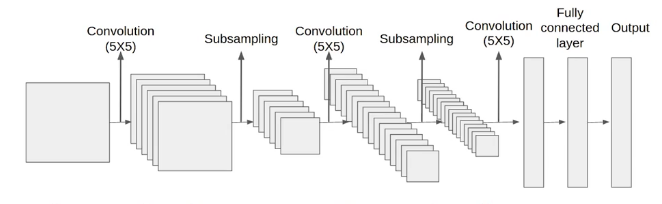
\includegraphics[width=\textwidth]{../presentation/lenet5.png}
  \caption{LeNet-5 Architecture.}
  \Description{description}
  \label{fig:teaser}
\end{teaserfigure}

%\received{20 February 2007}
%\received[revised]{12 March 2009}
%\received[accepted]{5 June 2009}

%%
%% This command processes the author and affiliation and title
%% information and builds the first part of the formatted document.
\maketitle

\section{Introduction}

text

INSPIRATION: https://www.nature.com/articles/s41598-020-79310-1 



\pagebreak
\section{Methods}

\subsection{Dataset}

The dataset for this project was obtained from the \href{https://www.congress.gov/members}{US Congress Members} archive. Photos of each member as well as their party affiliation (republican or democrat) were recorded. Members with an affiliation of ``independent'' were removed. After data collection, the rows were shuffled, and the dataset was split into training (80\%), validation (5\%) and testing (15\%). Images were also resized to 120 by 100 pixels (height by width) and converted to grayscale. Before CNN training, images were sequentially augmented thrice using the IMAGENET AutoAugment policy. 

\begin{figure}[h]
  \centering
  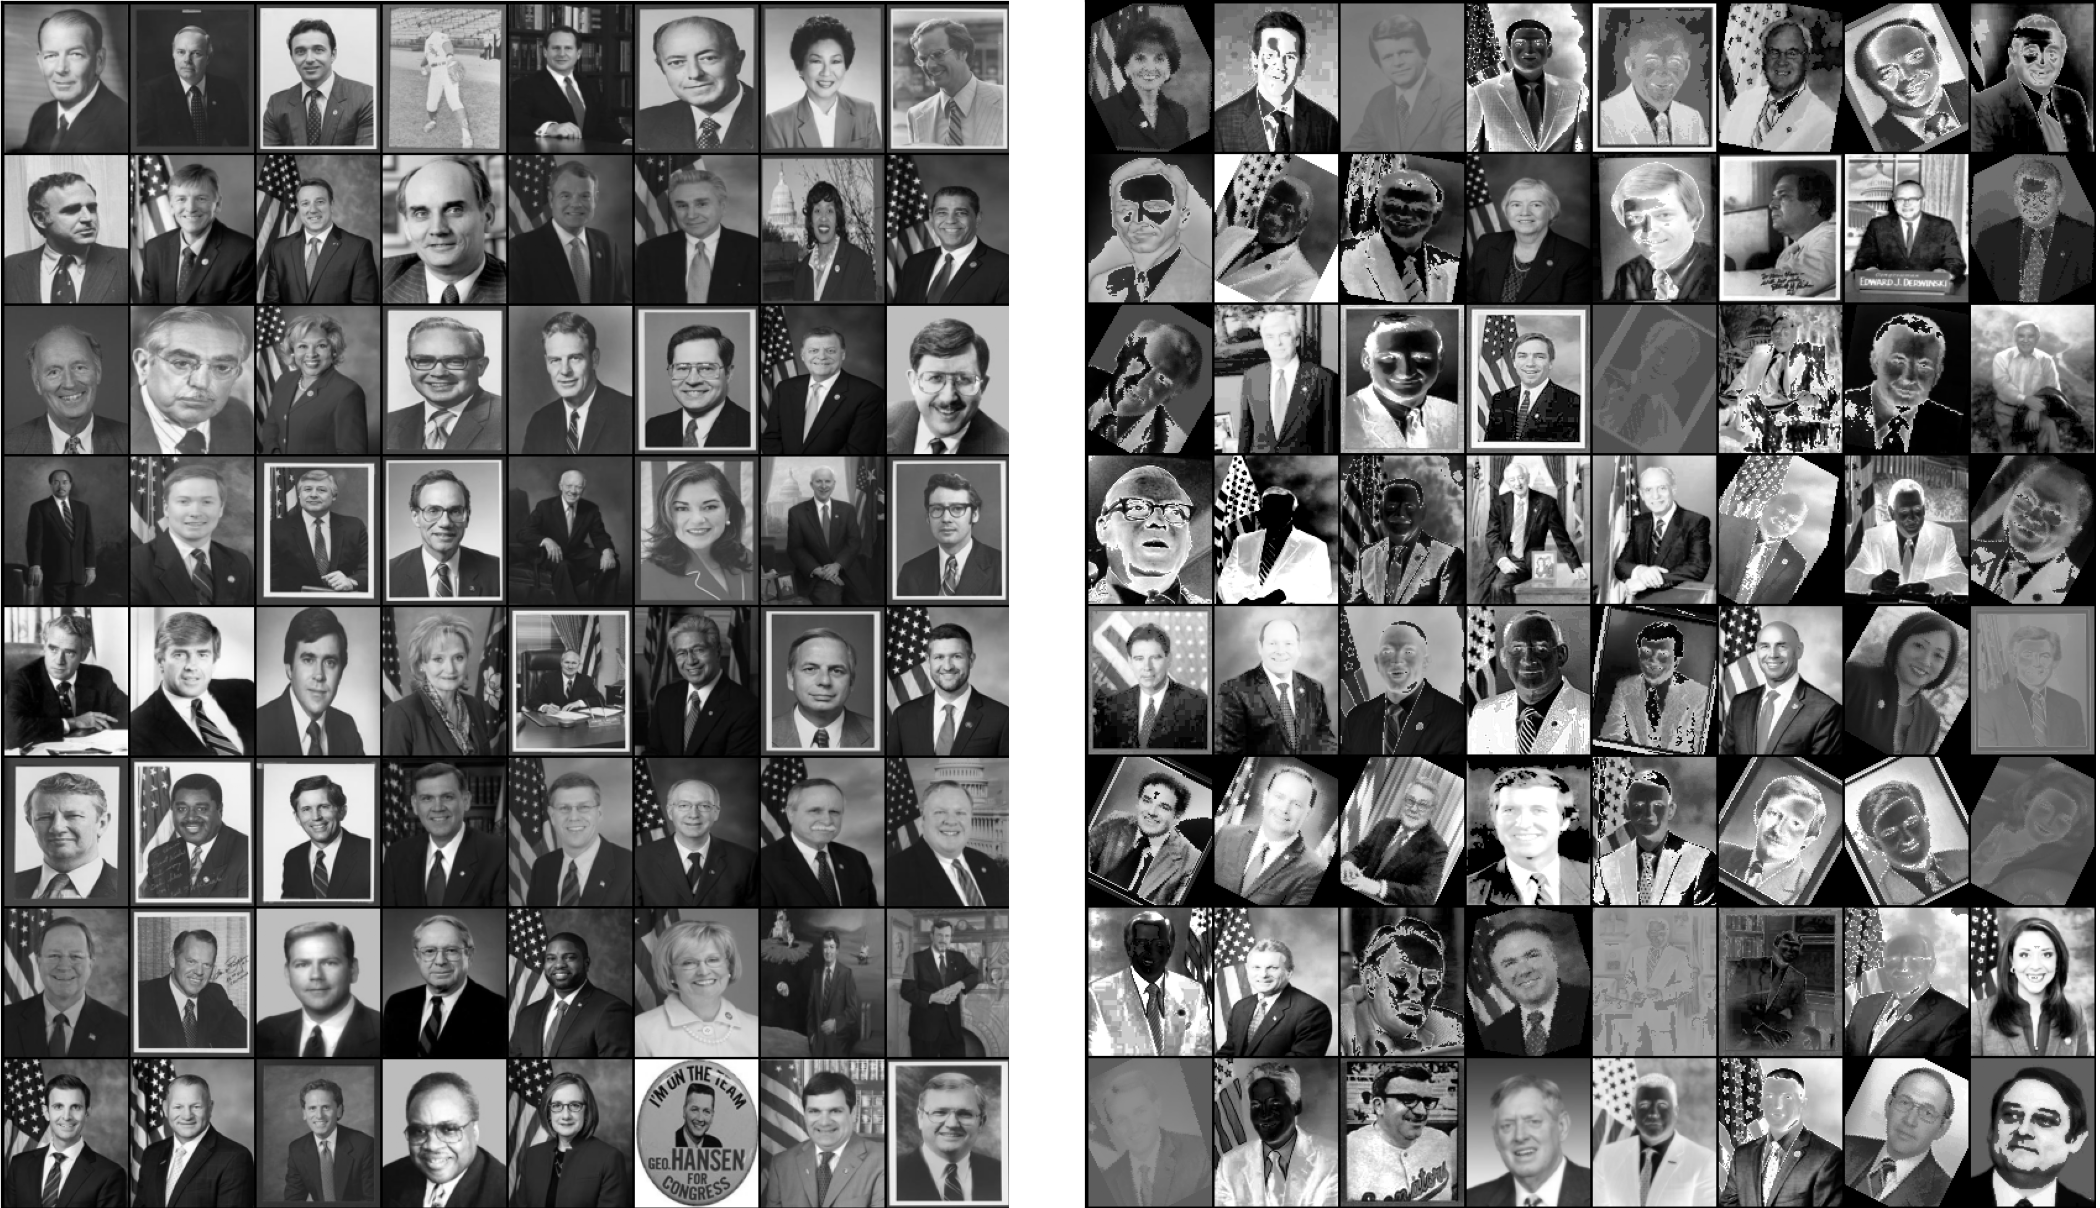
\includegraphics[width=\linewidth]{../presentation/batch_both.png}
  \caption{Left: A subset of one batch before augmentation (64/128). Right: A subset of one batch after image augmentation (64/128).}
  \label{fig:batch}
  \Description{text}
\end{figure}


\subsection{Architecture}

Three different architectures were trained and tested for classifying the images. These were LeNet-5, DenseNet, and a custom architecture (modified LeNet). The architectures of these NNs can be seen in \cref{tab:lenet5,tab:densenet,tab:custom}. The DenseNet architecture can be further investigated at \href{https://github.com/andreasveit/densenet-pytorch}{this GitHub repo}. 


\begin{table}[h!]
  \caption{}
  \label{tab:lenet5}
  \begin{tabular}{lcl}
    \textbf{LeNet-5} \\
    \toprule
    \textit{Features} \\
    \midrule
    Convolutional Layer &  & Kernel Size = 4 \\
    Tanh Activation & & \\
    Max Pooling Layer & & Kernel Size = 2\\
    Convolutional Layer &  & Kernel Size = 14 \\
    Tanh Activation & & \\
    Max Pooling Layer & & Kernel Size = 4\\
     & & \\
    \textit{Classifier} \\
    \midrule
    Linear & 1408 In & 120 Out\\
    Tanh Activation & & \\
    Dropout & & 0.7 \\
    Linear & 120 In & 84 Out\\
    Tanh Activation & & \\
    Dropout & & 0.8 \\
    Linear & 84 In & 2 Out\\
  \bottomrule
\end{tabular}
\end{table}


\begin{table}[h!]
\caption{}
  \label{tab:densenet}
  \begin{tabular}{lcl}
    \textbf{DenseNet} \\
    \toprule
    \textit{Features} \\
    \midrule
    Dense Block &  &  \\
    Transition Block & & \\
    Dense Block &  &  \\
    Transition Block & & \\
    Dense Block &  &  \\
    Batch Normalization & & \\
    \textit{Classifier} \\
    \midrule
    ReLU Activation &  & \\
    Linear & 24 In & 2 Out\\
    \bottomrule
\end{tabular}
\end{table}


\begin{table}[h!]
\caption{}
  \label{tab:custom}
  \begin{tabular}{lcl}
    \textbf{Modified LeNet-5 (Custom)} \\
    \toprule
    \textit{Features} \\
    \midrule
    Convolutional Layer &  & Kernel Size = 3 \\
    Sigmoid Activation & & \\
    Max Pooling Layer & & Kernel Size = 2\\
    Convolutional Layer &  & Kernel Size = 5 \\
    Sigmoid Activation & & \\
    Max Pooling Layer & & Kernel Size = 2\\
    Convolutional Layer &  & Kernel Size = 8 \\
    Sigmoid Activation & & \\
    Max Pooling Layer & & Kernel Size = 2\\
     & & \\
    \textit{Classifier} \\
    \midrule
    Linear & 1120 In & 120 Out\\
    Tanh Activation & & \\
    Dropout & & 0.8 \\
    Linear & 120 In & 84 Out\\
    Tanh Activation & & \\
    Dropout & & 0.6 \\
    Linear & 84 In & 2 Out\\
  \bottomrule
\end{tabular}
\end{table}


\subsection{Tuning}

Many tuning attempts were made in order to raise the classification rate for the test data. Learning rate, batch size, number of epochs, dropout rate, number of features, weight decay and depth (DenseNet only) were systematically altered. The best values for each hyperparameter were discovered for each of the models, and can be seen in \cref{tab:params}.

\begin{table}[h!]
\caption{}
  \label{tab:params}
  \begin{tabular}{lccc}
    \textbf{Hyperparameters} & LeNet-5 & DenseNet & Custom \\
    \toprule
    \textit{Learning Rate} & 0.001 & 0.0012 & 0.0015  \\
    \textit{Batch Size} & 128 & 128 & 128\\
    \textit{Epochs} & 12 & 15 & 15 \\
    \textit{Drop out} & 0.7, 0.8 & 0 & 0.8, 0.6 \\
    \textit{Features} & 12,000 & 12,000 & 12,000 \\
    \textit{Classes} & 2 & 2 & 2  \\
    \textit{Weight Decay} & 0.0002 & 0.0001 &  0.0001 \\
    \textit{Depth} & \textit{NA} & 4 & \textit{NA} \\
    \bottomrule
\end{tabular}
\end{table}










\section{Results}

The LeNet-5 model outperformed DenseNet and our custom LeNet by a significant margin, even after extensive tuning (\cref{fig:test}). LeNet-5 obtained a test classification rate of 60.21\%. DenseNet and custom LeNet achieved classification rates of 51.76\% and 51.51.41\%, respectively. These last two models perform only slightly better than random chance, while basic LeNet-5 performs decently well, but not amazing well. The convolutional filters of both convolutional layers for LeNet-5 can be seen in \cref{fig:filters}.
\par
Interestingly, \cref{fig:train,fig:valid} show that while all the models were able to converge to a solution on the training data, this convergence did not lead to better classification for the validation set. For the training data, all three models were able to converge to the minimum cost in only two epochs. In contrast, for the validation data, the models just seem to jump around without improving for all 15 epochs. 




\begin{figure}[h]
  \centering
  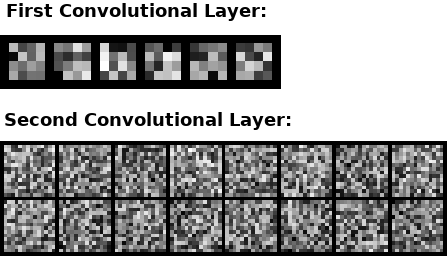
\includegraphics[width=\linewidth]{../presentation/filters.png}
  \caption{The convolutional filters of the first and second convolutional layers.}
  \label{fig:filters}
  \Description{text}
\end{figure}





\begin{figure}[h]
  \centering
  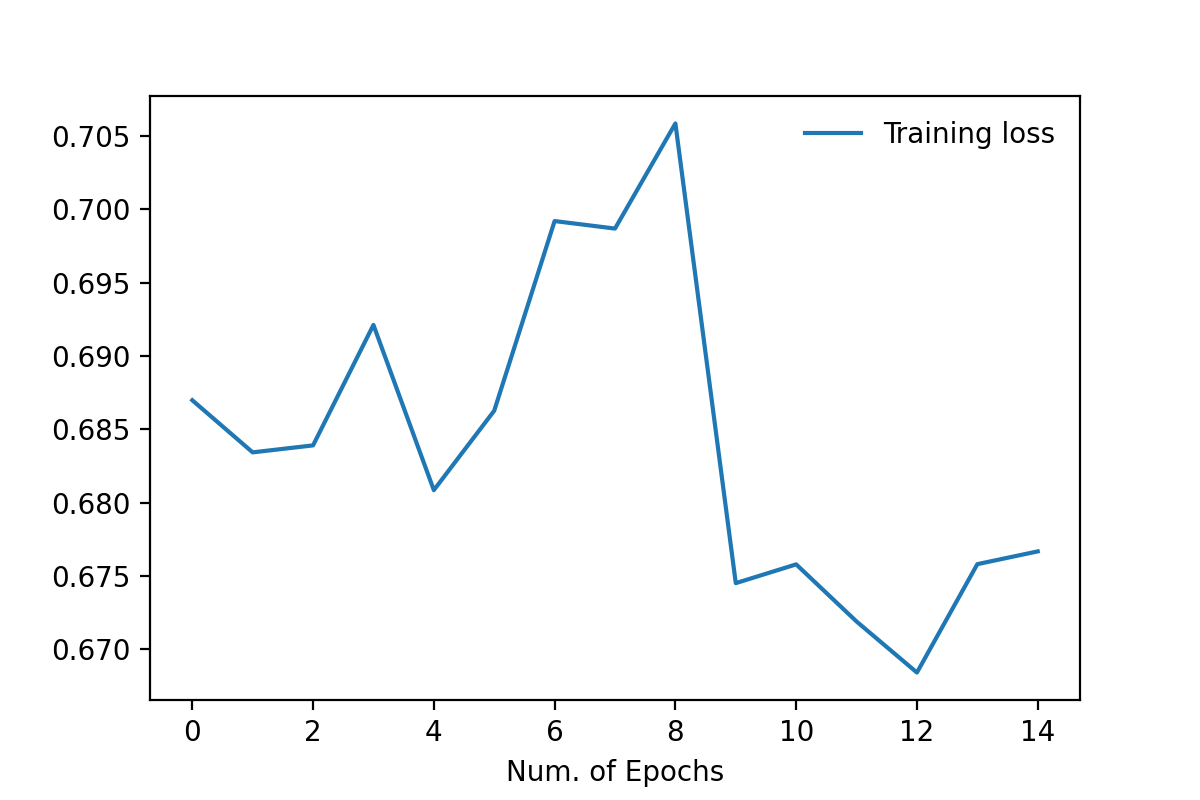
\includegraphics[width=\linewidth]{../presentation/training_cost.png}
  \caption{The training cost over 15 epochs for the 3 architectures considered.}
  \label{fig:train}
  \Description{text}
\end{figure}




\begin{figure}[h]
  \centering
  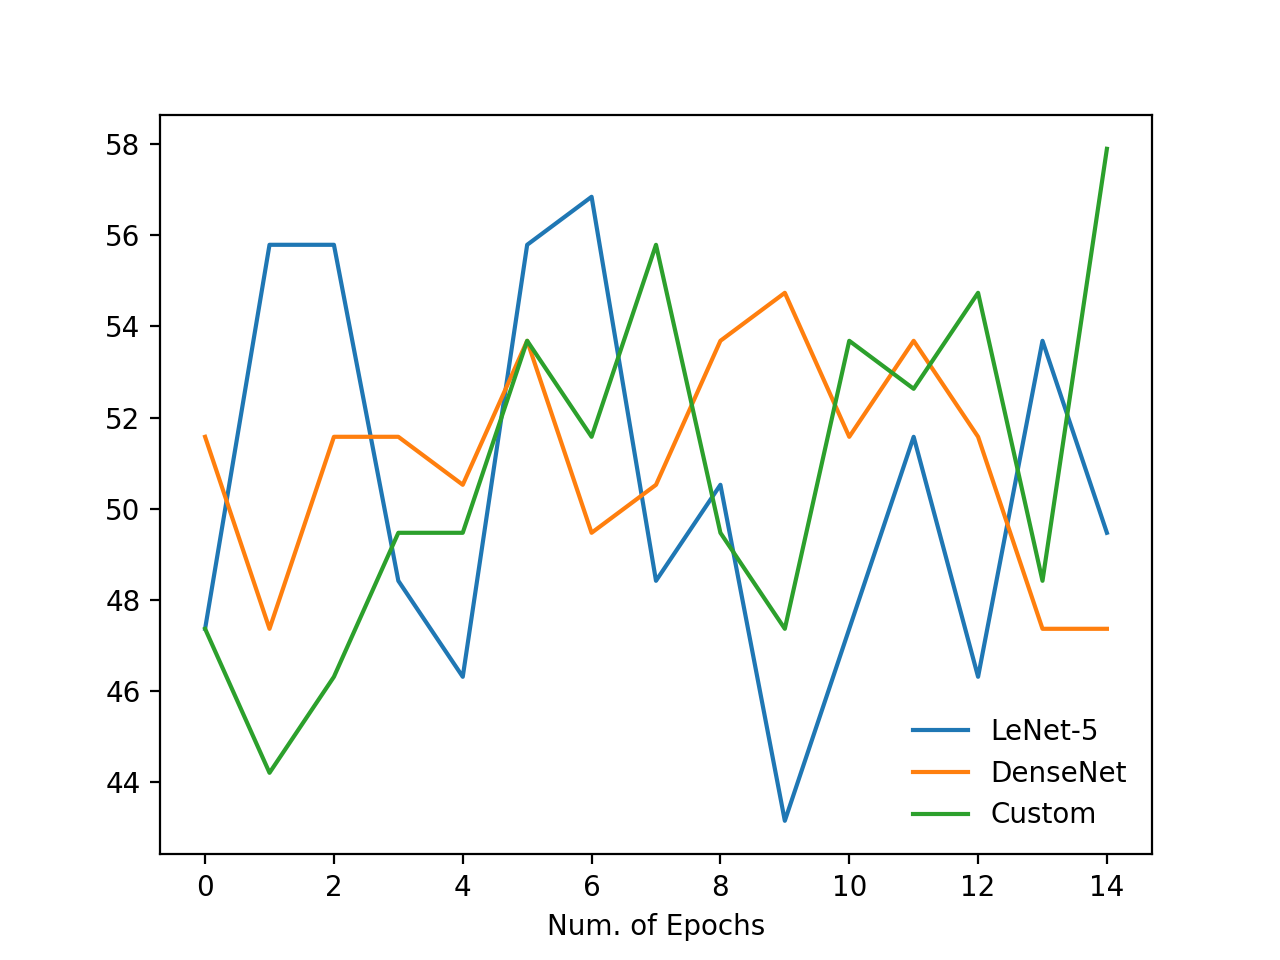
\includegraphics[width=\linewidth]{../presentation/validation_error.png}
  \caption{The validation error over 15 epochs for the 3 architectures considered.}
  \label{fig:valid}
  \Description{text}
\end{figure}






\begin{figure}[h]
  \centering
  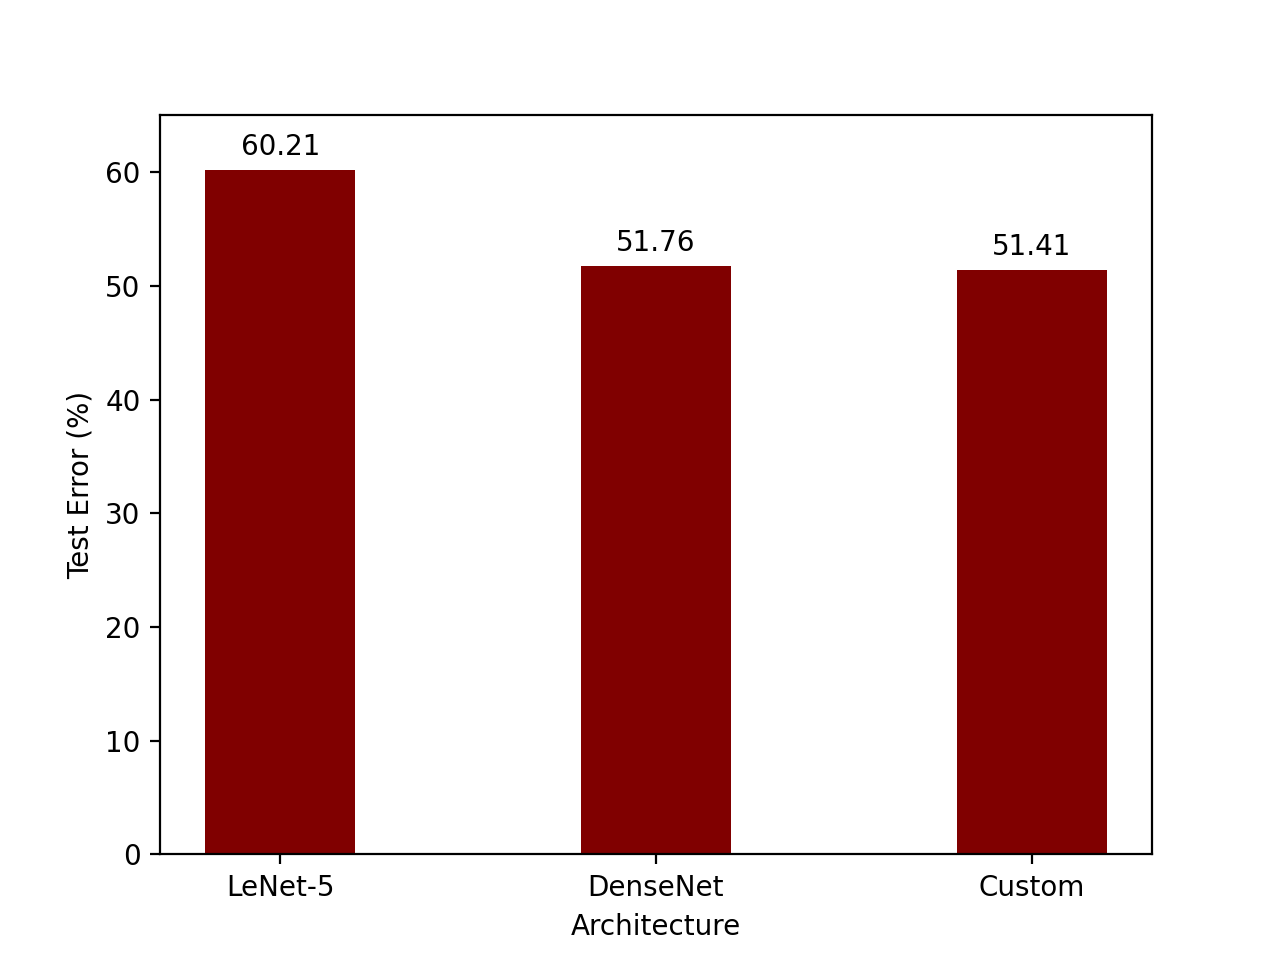
\includegraphics[width=\linewidth]{../presentation/finaltest_error.png}
  \caption{The final testing error for the 3 architectures considered.}
  \label{fig:test}
  \Description{text}
\end{figure}








\section{Discussion}


Mention why test class. rate is higher than train (bc train data is augmented/all messed up, testing data is not, so it's easier to classify the test images)


The poor classification rate of our NN may be to any of the following:

\begin{enumerate}
\item There is no actual difference in facial features between democrats and republicans. 
\item There are facial differences between democrats and republicans, but our dataset is too small to pick up on these subtle facial differences. 
\item The classifier section of the NN works well, but the convolution section is not properly picking up the meaningful facial features that are able to distinguish between the two parties. 
\item The convolution section of our NN is able to pick up on some meaningful signals, but the classification section is not performing well. 
\item The NN is only picking up features in the background of the image (and not the facial features), which are not predictive. 
\end{enumerate}

I think Number 5 is most likely. 




\section{Limitations \& Future Work}

Assumptions of this analysis due to the method of dataset construction are as follows:

\begin{itemize}
\item ``Democrats'' and ``republicans'' are good proxies for ``liberal'' and ``conservative'', respectively. 
\item Members of US congress are representative of democrats and republicans in general. 
\item Democrats and republicans have different facial attributes. 
\end{itemize}

In order to rectify the low classification rate of our NN, as well as to iron out the assumptions listed above, a new dataset should be collected. Ideally, the dataset would be collected from public social media profiles such as Facebook or dating websites. This new dataset should also be much larger, ideally by several orders of magnitude. Once this dataset is collected, more complex NN architectures could also be attempted. If this were to be done, we speculate that the classification rate would increase, as was seen in the Kosinski (2021) paper.




%%%%%%%%%%%%%%%%%%%%%%%%%%%%%%%%%%%%%%%%%%%%%%%%%%%%%%%%%%
\commentt{ %begin long comment out 
Immediately following this sentence is the point at which
Table~\ref{tab:freq} is included in the input file; compare the
placement of the table here with the table in the printed output of
this document.

\begin{table}
  \caption{Frequency of Special Characters}
  \label{tab:freq}
  \begin{tabular}{ccl}
    \toprule
    Non-English or Math&Frequency&Comments\\
    \midrule
    \O & 1 in 1,000& For Swedish names\\
    $\pi$ & 1 in 5& Common in math\\
    \$ & 4 in 5 & Used in business\\
    $\Psi^2_1$ & 1 in 40,000& Unexplained usage\\
  \bottomrule
\end{tabular}
\end{table}

To set a wider table, which takes up the whole width of the page's
live area, use the environment \textbf{table*} to enclose the table's
contents and the table caption.  As with a single-column table, this
wide table will ``float'' to a location deemed more
desirable. Immediately following this sentence is the point at which
Table~\ref{tab:commands} is included in the input file; again, it is
instructive to compare the placement of the table here with the table
in the printed output of this document.

\begin{table*}
  \caption{Some Typical Commands}
  \label{tab:commands}
  \begin{tabular}{ccl}
    \toprule
    Command &A Number & Comments\\
    \midrule
    \texttt{{\char'134}author} & 100& Author \\
    \texttt{{\char'134}table}& 300 & For tables\\
    \texttt{{\char'134}table*}& 400& For wider tables\\
    \bottomrule
  \end{tabular}
\end{table*}


\section{Figures}

The ``\verb|figure|'' environment should be used for figures. One or
more images can be placed within a figure. If your figure contains
third-party material, you must clearly identify it as such, as shown
in the example below.
\begin{figure}[h]
  \centering
  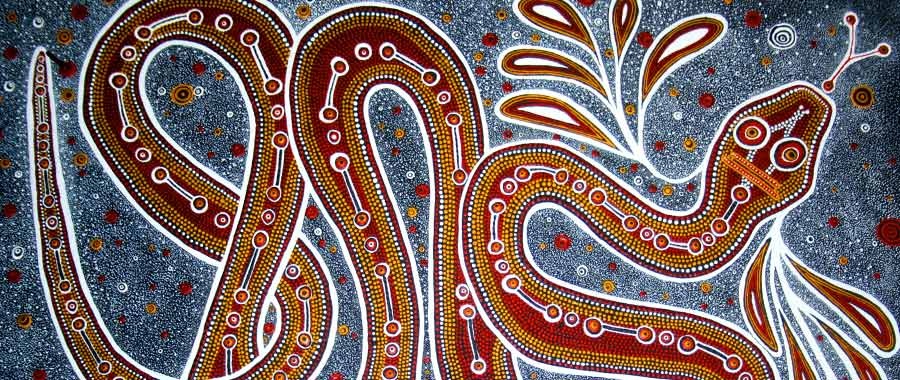
\includegraphics[width=\linewidth]{snake.jpg}
  \caption{1907 Franklin Model D roadster. Photograph by Harris \&
    Ewing, Inc. [Public domain], via Wikimedia
    Commons. (\url{https://goo.gl/VLCRBB}).}
  \Description{A woman and a girl in white dresses sit in an open car.}
\end{figure}

Your figures should contain a caption which describes the figure to
the reader.

Figure captions are placed {\itshape below} the figure.
}

\end{document}
\endinput
%%
%% End of file `sample-authordraft.tex'.
